\documentclass[12pt]{article}
\usepackage{times}
\usepackage{blindtext}
\usepackage{url}
\usepackage{float}

\usepackage{graphicx}
\graphicspath{{./figures/}}

\title{Observing the United States' Homelessness Crisis through Mathematical Methods}
\author{Mufaro Machaya, Nam Le, Ben Stilwell \\ Cy-Fair Senior High School \\ Cypress, Texas}
\date{March 3, 2024}


\begin{document}

\newpage

\section*{Executive Summary}
\blindtext

\maketitle
\newpage
\tableofcontents

\newpage

\section{Introduction}
Understanding the housing shortage has become more important than ever, as rates of homelessness have reached
unprecedented and potentially dire level\cite{NPR-ABGC-2022}. Moving into the future, it is
undeniably critical for promoting the general welfare of United States populations to best understand housing for
influencing public policy across major cities in the United States. Thus, we have prepared the following mathematical
models to best understand such a trend.

\newpage

\section{It was the Best of Times}

\subsection{Restatement of the Problem}
The first problem asks us to develop a mathematical model to predict changes to the housing supply over the next 50
years in two cities of our choosing: Seattle, Washington; and Albequerque, New Mexico.

\subsection{Assumptions and Justifications}

\textit{There will be no immense, drastic, and long-term permanent changes to housing production possibility
within the next fifty years.} \\

\noindent
Justification: Events that will drastically change the ability to produce housing, such as immense wars or widespread
natural disasters, are neigh-impossible to detect accurately with a simple mathematical model. The only events that can
be accurately tracked through mathematical means over short periods of time are cyclical events, like economic
recessions or inflation. \\

\noindent
\textit{Occupied housing will not be considered part of the available total housing supply.} \\

\noindent
Justification: In regards to fixing the homelessness crisis, housing that can be considered available for allocation to
unhoused people inherently must be unoccupied by others. \\

\noindent
\textit{Differences in median housing costs and median income per capita across regions in both Albequerque and Seattle
will not be considered in determining housing availability.} \\

\noindent
Justification: These factors hold a strong correlation with housing unavailability, yet we assume them to have no
causal relationship. \\

\subsection{Model Development}
For our housing availability model, we choose to use a simple vector machine that regresses historical housing availiability
data for both Albequerque and Seattle, and from there, we cross-reference this data with historical economic trends
across the United States to best model housing availability over time given cyclical economic trends.

\noindent
To begin, we trained the model on the following datasets for housing availability in Albequerque and Seattle and the
national GDP of the United States.

\begin{table}[H]
  \centering
  \begin{tabular}{|c c c c|} 
    \hline 
    Year & Total housing units & Occupied units & Vacant units \\ [0.5ex]
    \hline
    2010  &  234,891 & 217,256 & 17,635 \\
    2011  &  237,735 & 220,060 & 17,675 \\
    2012  &  239,718 & 222,584 & 17,134 \\
    2013  &  240,277 & 222,491 & 17,786 \\
    2014  &  240,961 & 222,868 & 18,093 \\
    2015  &  241,326 & 222,098 & 19,228 \\
    2016  &  242,070 & 221,320 & 20,750 \\
    2017  &  243,402 & 221,119 & 22,283 \\
    2018  &  244,382 & 222,748 & 21,634 \\
    2019  &  245,476 & 224,166 & 21,310 \\
    2020  &  247,926 & 229,701 & 18,225 \\
    2021  &  252,924 & 236,191 & 16,733 \\
    2022  &  255,178 & 239,800 & 15,378 \\ [1ex] 
    \hline
  \end{tabular}
  \caption{Housing Statistics in Albequerque, New Mexico \cite{Census2010ACSDP1Y2010.DP04}.}
\end{table}

\begin{table}[H]
  \centering
  \begin{tabular}{|c c c c|}
    \hline
    Year & Total housing units & Occupied units & Vacant units \\ [0.5ex]
    \hline
    2010 & 302,465 & 280,453 & 22,012 \\
    2011 & 304,164 & 282,480 & 21,684 \\
    2012 & 306,694 & 285,476 & 21,218 \\
    2013 & 309,205 & 288,439 & 20,766 \\
    2014 & 311,286 & 290,822 & 20,464 \\
    2015 & 315,950 & 296,633 & 19,317 \\
    2016 & 322,795 & 304,157 & 18,638 \\
    2017 & 334,739 & 314,850 & 19,889 \\
    2018 & 344,503 & 323,446 & 21,057 \\
    2019 & 354,475 & 331,836 & 22,639 \\
    2020 & 367,337 & 344,629 & 22,708 \\
    2021 & 362,809 & 337,361 & 25,448 \\
    2022 & 372,436 & 345,246 & 27,190 \\ [1ex]
    \hline
  \end{tabular}
  \caption{Housing Statistics in Seattle, Washington \cite{Census2010ACSDP5Y2010.DP04}.}
\end{table}

\noindent
Due to the limited size of the dataset, we chose to use a $C$ value for our SVM closer to 1.0 to prevent overfitting or
underfitting of the data. 

\begin{figure}[H]
  \centering
  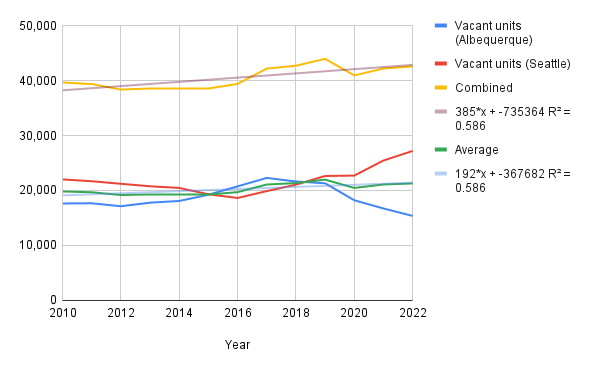
\includegraphics[width=0.9\textwidth]{vacancy}
  \caption{The number of vacancies in Albequerque and Seattle from 2010 to 2022 \cite{Census2010ACSDP1Y2010.DP04,Census2010ACSDP5Y2010.DP04}.}
\end{figure}

\noindent
Let $H(x)$ equal the number of available houses for a given year, where $x$ is the current year (absolute from year 0, such as 2024). Simple regression on this dataset results in a total trendline of

$$H_{\textrm{\small TOTAL}}(x) = 385x - 735,364$$

\noindent
where $R^{2}_{\textrm{\small TOTAL}} = 0.586$, and an average trendline of

$$H_{\textrm{\small AVG}}(x) = 192x - 367,682$$

\noindent
where $R^{2}_{\textrm{\small AVG}} = 0.586$. \\

\noindent
A coefficient of determination of $0.586$ is undeniably subpar due to the immense indifficulty in representing vast differences across the trends with linear functions.

\subsection{Results}

With this model, we can predict the following housing statistics for 2034 (10 years in the future), 2044 (20 years in the future), and 2074 (50 years in the future):

\begin{table}[H]
  \centering
  \begin{tabular}{|c c|c c c|}
    \hline 
    &&&&\\
    Year & \shortstack{Years from 2024} & \shortstack{Total Available \\ Homes} & \shortstack{Average Available \\ Homes in Each \\ City} & \shortstack{Change from 2024} \\
    \hline
    2024 & 0  & 43,876 & 20,926 & 0 \\
    2034 & 10 & 47,726 & 22,846 & 1,920 \\
    2044 & 20 & 51,576 & 24,766 & 1,920 \\
    2074 & 50 & 63,126 & 30,526 & 1,920 \\
    \hline
  \end{tabular}
\end{table}

\subsection{Reflecting on the Model}

Overall, our model proves generally weak at predicting immense, unforseen changes to the economic situation of both cities such as the advent of war, the outbreak of a major epidemic/pandemic, or a large-scale natural disaster. This model is best for serving as a general, aggregate predictor of housing availability based on cyclical economic trends. Our coefficient of determination $R^{2}$ is certainly low, indicating a lack of accuracy, but this is certainly due to the difficulty of modeling previously-mentioned large-scale events with a linear model. \\ 

\noindent
Altogether, we can conclude that this model's impact serves best as a general guideline for understanding realistic public policy because it is solely based largely on aggregate, cyclical economic factors that can be reasonably relied upon to occur continuously.

\newpage

\section{It was the Worst of Times}

\subsection{Restatement of the Problem}
The first problem asks us to develop a mathematical model to predict changes to the homeless population over the next 50
years in two cities of our choosing: Seattle, Washington; and Albequerque, New Mexico.

\subsection{Assumptions and Justifications}
\textit{Public policy regarding homelessness will stay roughly the same throughout the next fifty years.} \\

\noindent
Justification: We assume that there will be no significant changes to government policy that would severely change the homeless population, as these immense changes to public policy require immense predictions of political trends beyond the scope of this study. \\

\subsection{Model Development}
For our model, we used yet another linear support vector machine for simple linear regression at $C=1.0$ as trained on the following data sets:

\begin{table}[H]
  \centering
  \begin{tabular}{|c c c c|} 
    \hline 
    Year & Total housing units & Occupied units & Vacant units \\ [0.5ex]
    \hline
    2010 & 234,891 & 217,256 & 17,635 \\
    2011 & 237,735 & 220,060 & 17,675 \\
    2012 & 239,718 & 222,584 & 17,134 \\
    2013 & 240,277 & 222,491 & 17,786 \\
    2014 & 240,961 & 222,868 & 18,093 \\
    2015 & 241,326 & 222,098 & 19,228 \\
    2016 & 242,070 & 221,320 & 20,750 \\
    2017 & 243,402 & 221,119 & 22,283 \\
    2018 & 244,382 & 222,748 & 21,634 \\
    2019 & 245,476 & 224,166 & 21,310 \\
    2020 & 247,926 & 229,701 & 18,225 \\
    2021 & 252,924 & 236,191 & 16,733 \\
    2022 & 255,178 & 239,800 & 15,378 \\ [1ex] 
    \hline
  \end{tabular}
  \caption{Housing Statistics in Albequerque, New Mexico \cite{Census2010ACSDP1Y2010.DP04}.}
\end{table}

\begin{figure}[H]
  \centering
  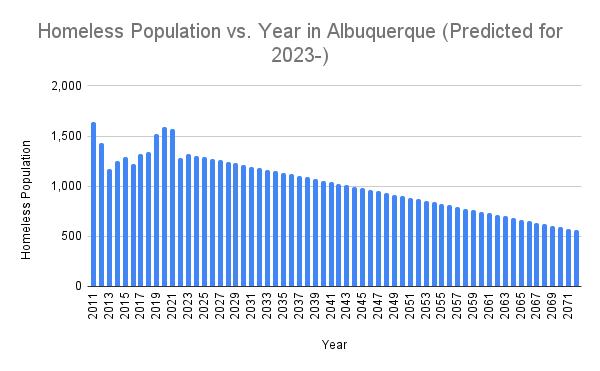
\includegraphics[width=0.8\textwidth]{homeless-vs-year-alb}
  \caption{Total Homeless by Year in Albequerque, New Mexico}
\end{figure}

\begin{figure}[H]
  \centering
  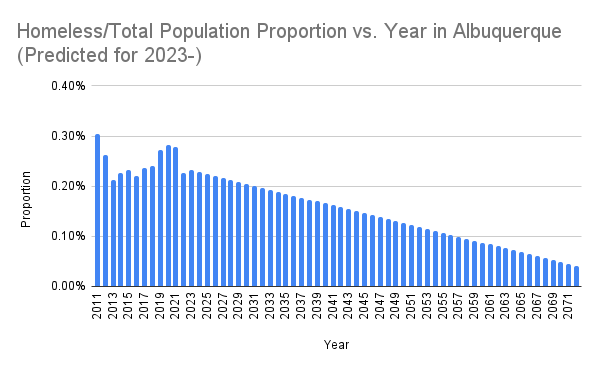
\includegraphics[width=0.8\textwidth]{homeless-prop-vs-year-alb}
  \caption{Percentage of the Population that is Homeless in Albequerque, New Mexico}
\end{figure}

\noindent
Therefore, for Albequerque, let $A_{T}(x)$ be total number of homeless people in Albequerque, where $x$ is the current year (which is absolute from 0, such as 2024).

$$A_{T}(x) = 32,757.7 - 15.54(x)$$

\noindent
Additionally, let $A_{\%}(x)$ be the percentage of Albequerque's population that is homeless, where $x$ is the current year (which is absolute from 0, such as 2024).

$$A_{\%}(x) = .08124 - 3.9(x) \times 10^{-5}$$

\begin{figure}[H]
  \centering
  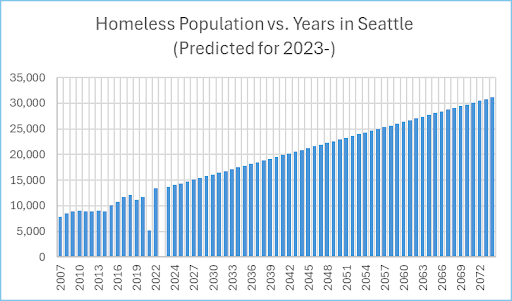
\includegraphics[width=0.8\textwidth]{homeless-vs-year-seattle}
  \caption{Total Homeless by Year in Seattle, Washington}
\end{figure}

\begin{figure}[H]
  \centering
  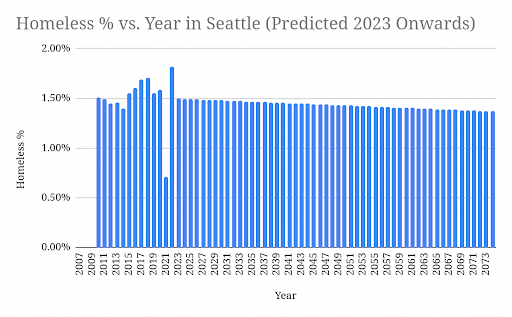
\includegraphics[width=0.8\textwidth]{homeless-prop-vs-year-seattle}
  \caption{Percentage of the Population that is Homeless in Seattle, Washington}
\end{figure}

\noindent
Therefore, for Seattle, let $S_{T}(x)$ be total number of homeless people in Seattle, where $x$ is the current year (which is absolute from 0, such as 2024).

$$S_{T}(x) = 341.625x + 7902$$

\noindent
Additionally, let $S_{\%}(x)$ be the percentage of Seattle's population that is homeless, where $x$ is the current year (which is absolute from 0, such as 2024).

$$S_{\%}(x) = 0.65 - 2.473(x) \times 10^{-5}$$

\subsection{Results}

With this model, we can predict the following homelessness statistics for 2034 (10 years in the future), 2044 (20 years in the future), and 2074 (50 years in the future):

\subsubsection{Albequerque, New Mexico}

\begin{table}[H]
  \centering
  \begin{tabular}{|c c|c c c|}
    \hline 
    Year & \shortstack{Years from 2024} & \shortstack{Homeless Percentage} & \shortstack{Total Homeless} & \shortstack{Change from 2024} \\
    \hline
    $2024$ & $0$  & $2.304 \times 10^{-3}$ & $1,304.74$ & $0$ \\
    $2034$ & $10$ & $1.914 \times 10^{-3}$ & $1,149.34$ & $-155.4$ \\
    $2044$ & $20$ & $1.524 \times 10^{-3}$ & $993.94$   & $-155.4$ \\
    $2074$ & $50$ & $3.54  \times 10^{-3}$ & $527.74$   & $-155.4$ \\
    \hline
  \end{tabular}
\end{table}

\subsubsection{Seattle, Washington}

\begin{table}[H]
  \centering
  \begin{tabular}{|c c|c c c|}
    \hline 
    Year & \shortstack{Years from 2024} & \shortstack{Homeless Percentage} & \shortstack{Total Homeless} & \shortstack{Change from 2024} \\
    \hline
    $2024$ & $0$  & $0.6$   & $699,351$    & $0$ \\
    $2034$ & $10$ & $0.6$   & $702,767.25$ & $3,416.25$ \\
    $2044$ & $20$ & $0.6$   & $706,183.5$  & $3,416.5$ \\
    $2074$ & $50$ & $0.599$ & $716,432.25$ & $10,249$ \\
    \hline
  \end{tabular}
\end{table}

\subsection{Reflecting on the Model}

Reflecting on the Models: Our homeless models for both the city of Seattle and Albuquerque proves a little weak, as the homeless population rate won’t have a linear decrease or increase following the year 2023, but will have its ups and downs. Although our data for the graphs are not perfect, it offers a distinct trend between the two cities, since Seattle’s estimated homeless population rate is going up, while Albuquerque’s homeless population rate is going down. This gives insight on the effectiveness of Albuquerque’s methods in solving the homeless crisis, and should be explored furthermore.

\newpage

\section{Rising from this Abyss}

\subsection{Restatement of the Problem}
\subsection{Assumptions and Justifications}
\subsection{Model Development}
\subsection{Results}
\subsection{Reflecting on the Model}

\newpage

\Urlmuskip=0mu plus 1mu\relax
\bibliographystyle{plain}
\bibliography{sources}

\end{document}
